\chapter{Software Requirements Specification}
\label{ch:srs}
This chapter will contain the functional and non-functional requirements of the project.
\section{List of functions}
List of key features for the "Improving Medical Education through Immersive Virtual Reality (MetaMed)" project:\\
\textbf{Realistic medical simulations:}\\ Create highly realistic medical scenarios and procedures that faithfully mimic real medical experiences, including various medical specialties.\\
\textbf{Haptic feedback integration:}\\ Integrate tactile feedback devices to provide tactile sensations, increasing the realism of medical training and allowing students to develop their tactile skills.\\
\textbf{Immersive 3D Environments:}\\ Create immersive, 3D virtual environments that accurately represent medical settings, including operating rooms, medical instruments, and anatomical structures.\\
\textbf{Interactivity:}\\Enables hands-on interaction with virtual medical tools, instruments, and equipment, allowing students to perform medical tasks and procedures.\\
\textbf{Remote Access:}\\ Enable medical students to access a metaverse-based medical training platform from remote locations, facilitating flexible learning.
\section{Test plan (test level, test techniques)}
\text{Test plan for our project will be as:}
\begin{itemize}
    \item Movement in VR 
    \item Interaction with Objects
    \item Treatement to Patient
\end{itemize}
\section{Use Case Diagram}
Here is the Use Case Diagram of the Project.
\begin{figure}[h]
    \centering
    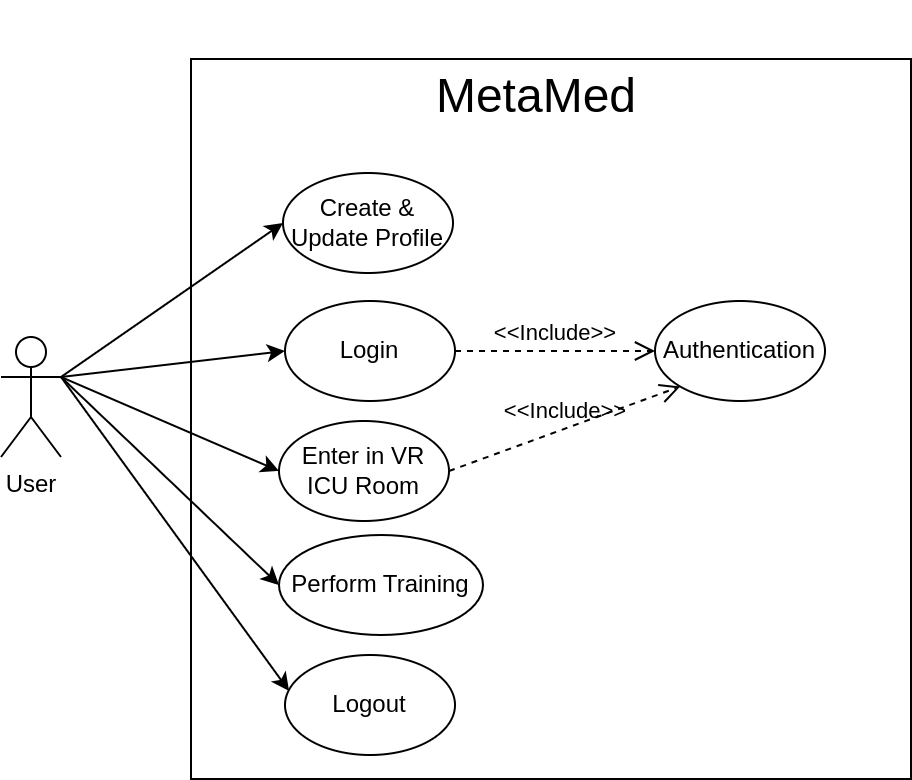
\includegraphics[width=0.6\textwidth, height=0.3\textheight]{Images/Use Case.drawio.png}
    \caption{Use Case Diagram}
    \label{fig:system-diagram}
\end{figure}

\section{Software Development Plan}
\text{Software Development Plan for our project will be as:}
\begin{itemize}
    \item Project Overview 
    \item Requirements Gathering and Analysis
    \item System Design
    \item Development
    \item Testing
    \item Documentation
    \item Management
\end{itemize}

\section{System Diagram}
It is the System Diagram of the Project.
\begin{figure}[h]
    \centering
    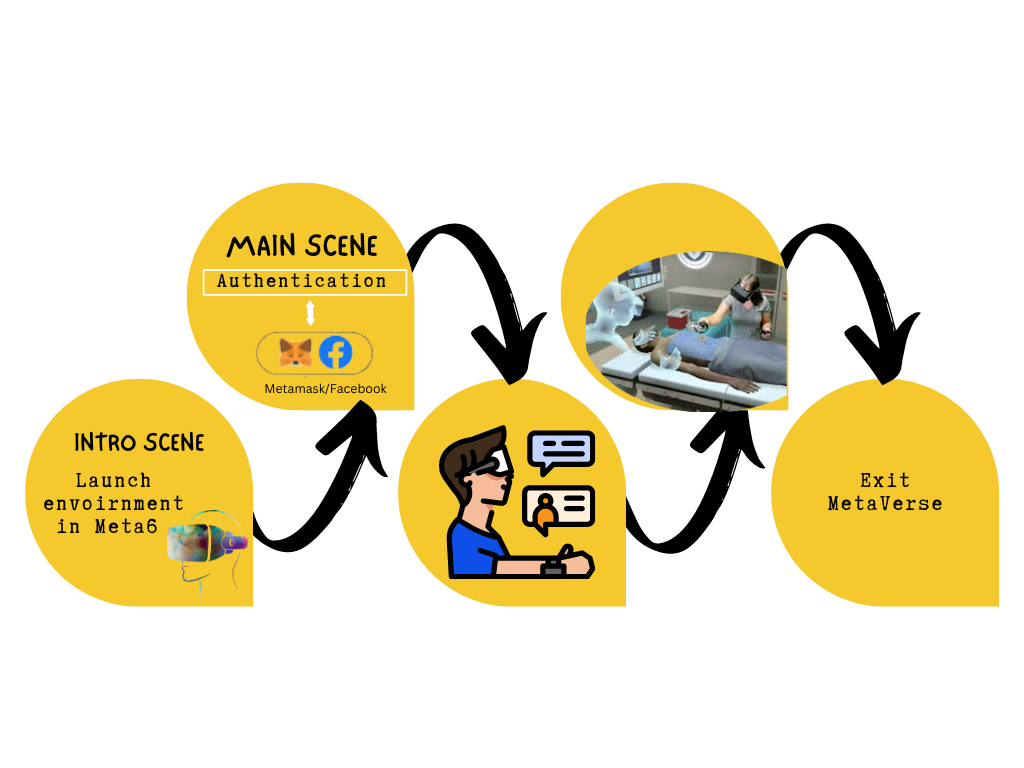
\includegraphics[width=1\linewidth, height=0.65\linewidth]{Images/system.png}
    \caption{System Diagram}
\end{figure}
\newpage
\section{Activity Daigram}
The activity diagram aims to illustrate the entire process of project working and demonstration.
\begin{figure}[h]
    \centering
    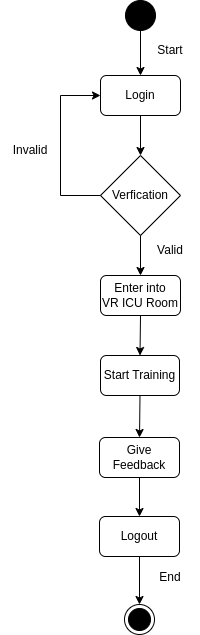
\includegraphics[width=0.25\linewidth]{Images/Activity.drawio.png}
    \caption{Activity Diagram}
\end{figure}
\newpage
\section{Tools and Technologies used}
These are some tools and technologies used in this project.
\subsection{C-Sharp:}
C-sharp is a programming language developed by Microsoft for use with the .NET Framework. It is widely used for developing web applications, desktop applications, mobile apps, games, and more. Known for its versatility and ease of use, C-sharp is popular in various software development fields. It supports object-oriented programming and provides a rich set of libraries, making it a powerful tool for developers.
%\begin{figure}[h]
%	\centering
%	
\includegraphics[width=0.1\linewidth, height=0.1\linewidth]{Images/CSharp.png}
%	\caption{C-Sharp\cite{csharp}}
%\end{figure}
\subsection{Blender}
Blender is a free, open-source 3D graphics software used for creating a wide range of visual content, including animated films, visual effects, art, and models. It also supports motion graphics, interactive applications, and virtual reality. Blender's versatility makes it popular among artists, animators, and developers. Its open-source nature allows for community-driven improvements and extensive customization. Blender is a powerful tool in the 3D graphics industry.
%\begin{figure}[h]
%	\centering
%	
\includegraphics[width=0.2\linewidth, height=0.2\linewidth]{Images/blender.png}
%	\caption{blender\cite{blender}}
%\end{figure}
\subsection{Git}
Git is a distributed version control system that tracks versions of files. It is used to control source code and collaboratively developing software. Git is a distributed version control system that efficiently manages and tracks changes in projects of any size. Created by Linus Torvalds in 2005, Git allows every developer to have a full copy of the project’s history, making it resilient and suitable for offline work.
%\begin{figure}[h]
%	\centering
%	
\includegraphics[width=0.15\linewidth, height=0.15\linewidth]{Images/git.png}
%	\caption{git\cite{git-logo}}
%\end{figure}
\newpage
\subsection{GitHub}
GitHub is a platform for developers to create, store, manage, and share their code, utilizing Git for distributed version control. It offers features like access control, task management, and continuous integration, making it a central hub for collaborative software development. GitHub facilitates project collaboration, allowing multiple contributors to work on the same codebase seamlessly. Its integration with Git ensures that changes are tracked, and the development process is efficient and organized.
%\begin{figure}[h]
%	\centering
%	
\includegraphics[width=0.1\linewidth, height=0.1\linewidth]{Images/GitHub.png}
%	\caption{GitHub\cite{github-logo}}
%\end{figure}
\subsection{Meta}
The Metaverse is a sophisticated, interconnected virtual world that enhances user experiences by offering seamless, immersive digital environments. It merges physical and virtual realities, allowing users to interact, work, and play within a shared, persistent digital space. This virtual universe encompasses everything from social interactions to business activities, powered by technologies like virtual reality (VR), augmented reality (AR), and blockchain. As the Metaverse evolves, it is expected to transform how we engage with digital content and each other, creating new opportunities for innovation and connection.
%\begin{figure}[h]
%	\centering
%	
\includegraphics[width=0.2\linewidth, height=0.2\linewidth]{Images/meta.png}
%	\caption{Meta\cite{meta}}
%\end{figure}
\subsection{Unity}
Unity is a versatile engine used for developing both 3D and 2D games, as well as interactive simulations. Its flexibility and user-friendly interface have led to widespread adoption across various industries beyond video gaming, including film, automotive, architecture, and education. Unity supports a range of platforms, enabling developers to create cross-platform applications with ease. Its robust asset store and strong community support make it a popular choice for creating immersive and engaging digital experiences.
%\begin{figure}[h]
%	\centering
%	
\includegraphics[width=0.2\linewidth,height=0.2\linewidth]{Images/unity.png}
%	\caption{Unity\cite{Unity}}
%\end{figure}
\newpage
\subsection{Meta Quest 2}
Project MetaMed VR used the Meta Quest 2 to leverage its advanced features such as hand tracking and gesture recognition, significantly enhancing medical education through immersive virtual reality experiences. The Meta Quest 2's capabilities provide a more interactive and engaging learning environment, allowing users to practice and visualize complex medical procedures in a virtual space. This innovative approach helps bridge the gap between theoretical knowledge and practical application, making medical training more effective and accessible.
%\begin{figure}[h]
%	\centering
%	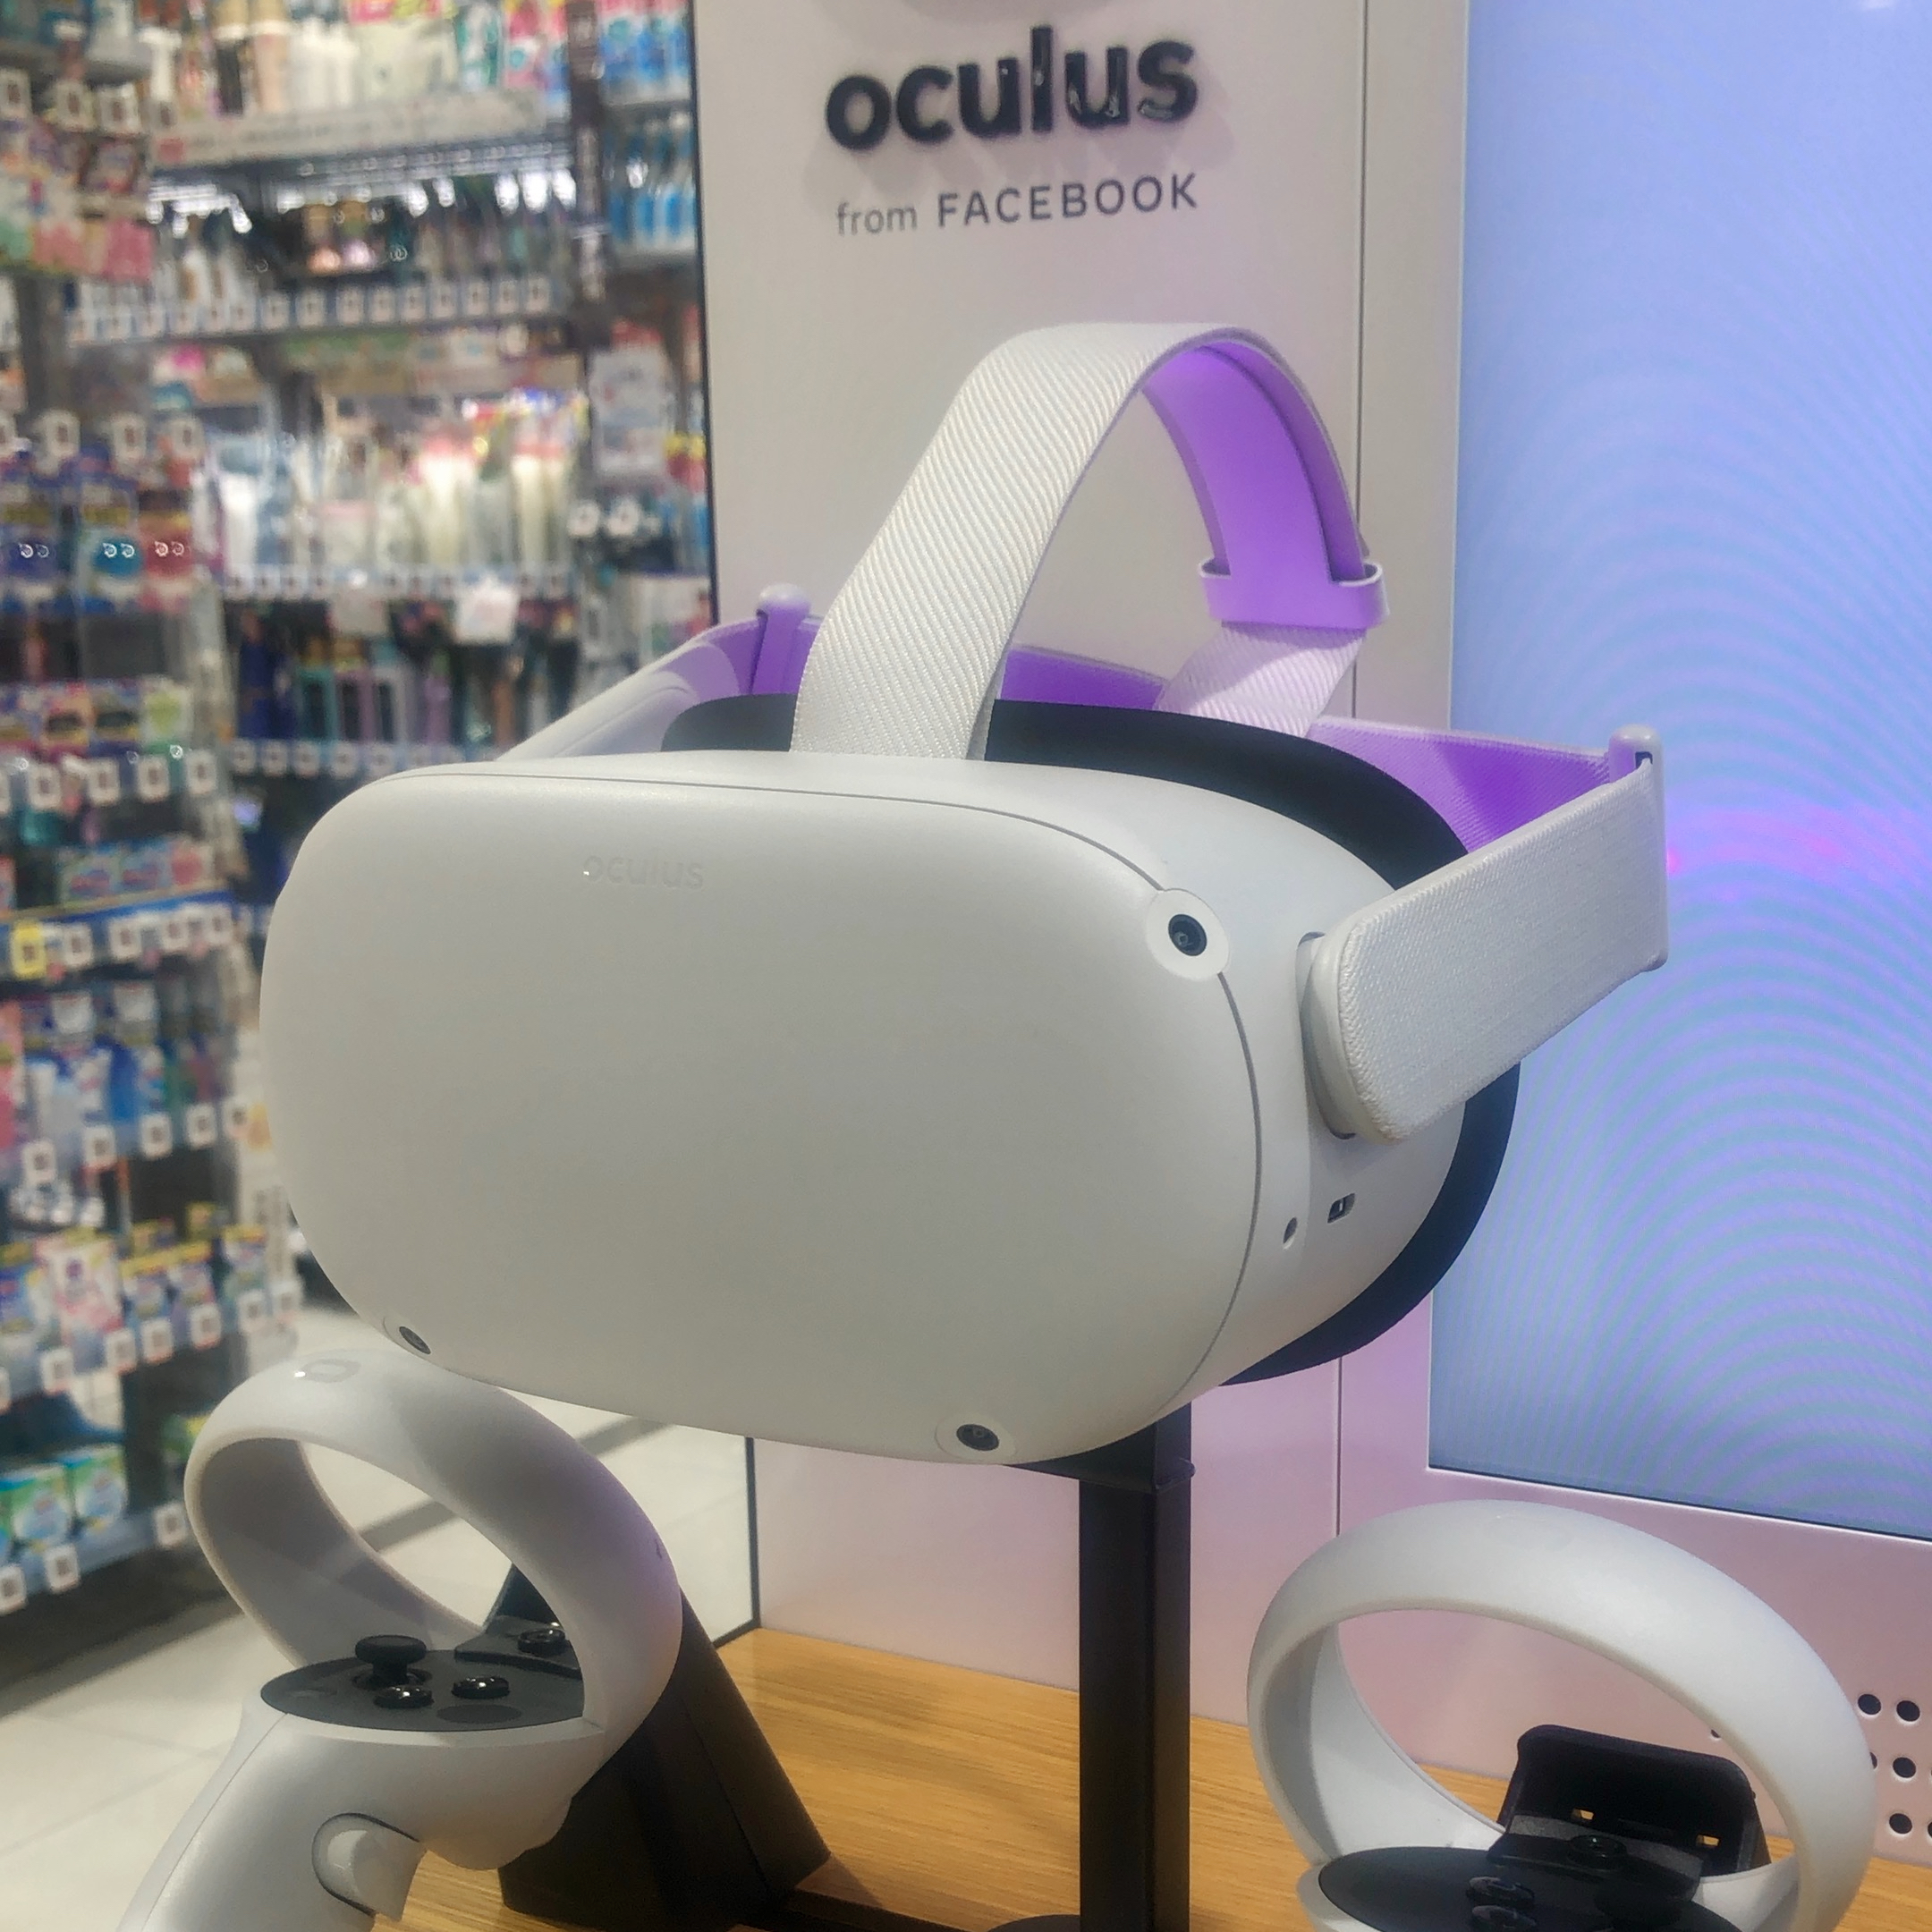
\includegraphics[width=0.4\linewidth,height=0.3\linewidth]{Images/metaquest2.png}
%	\caption{Meta Quest 2\cite{metaquest}}
%\end{figure}
\subsection{Microsoft Visual C++}
Microsoft Visual C++ is integrated with Unity 3D to optimize code, enhance performance, and manage memory in complex applications. This integration ensures smooth and efficient gameplay by providing advanced debugging, profiling, and optimization tools. Visual C++ helps developers address performance bottlenecks and memory management issues, which is crucial for creating high-quality, resource-intensive games and applications. By leveraging these capabilities, Unity developers can achieve better overall performance and stability in their projects.
%\begin{figure}[h]
%	\centering
%	
\includegraphics[width=0.2\linewidth,height=0.2\linewidth]{Images/VS Code.png}
%	\caption{Microsoft Visual C++\cite{visual-studio-icon}}
%\end{figure}